%\section{Design Rationale}
%\subsection{Design Challenges}
%
%\pandora faces three key challenges.
%(1) The sample selection strategy deployed in CDA-AL restricts the arbitrary injection of poisoned samples into the training data.
%Therefore, attackers must ensure that the victim model selects poisoned samples for labeling.
%(2) The sample labeling process in active learning is based on manual analysis, meaning the labels of all poisoned samples in the training data must remain correct.
%The attacker cannot degrade the victim model’s concept drift adaptation performance by tampering with the sample labels~\cite{2018-NIPS-Poison-frogs,2019-NIPS-Transferable-clean-label-poisoning-attacks-on-deep-neural-nets}.
%(3) Existing targeted poisoning attacks are typically evaluated for effectiveness on models with fixed parameters. 
%For example, backdoor attacks are often evaluated on pre-trained models~\cite{2024-TIFS-Backdoor-Contrastive-Learning,2021-Usenix-Poisoning-Attack-Explanation-guided-Backdoor,2023-SP-backdoor-attack}.
%In contrast, \pandora must ensure its attack remains effective as the victim model continuously updates its parameters.
%\pandora tackles the first two challenges.
%The final challenge is addressed through continuous attacks on the concept drift adaptation process.
%Additionally, we validate the persistence of the attack’s effectiveness on concept drift data spanning seven years, as discussed in Section~\ref{Sec: Single Attack Targets}.


\begin{figure}[t]
	\centering
	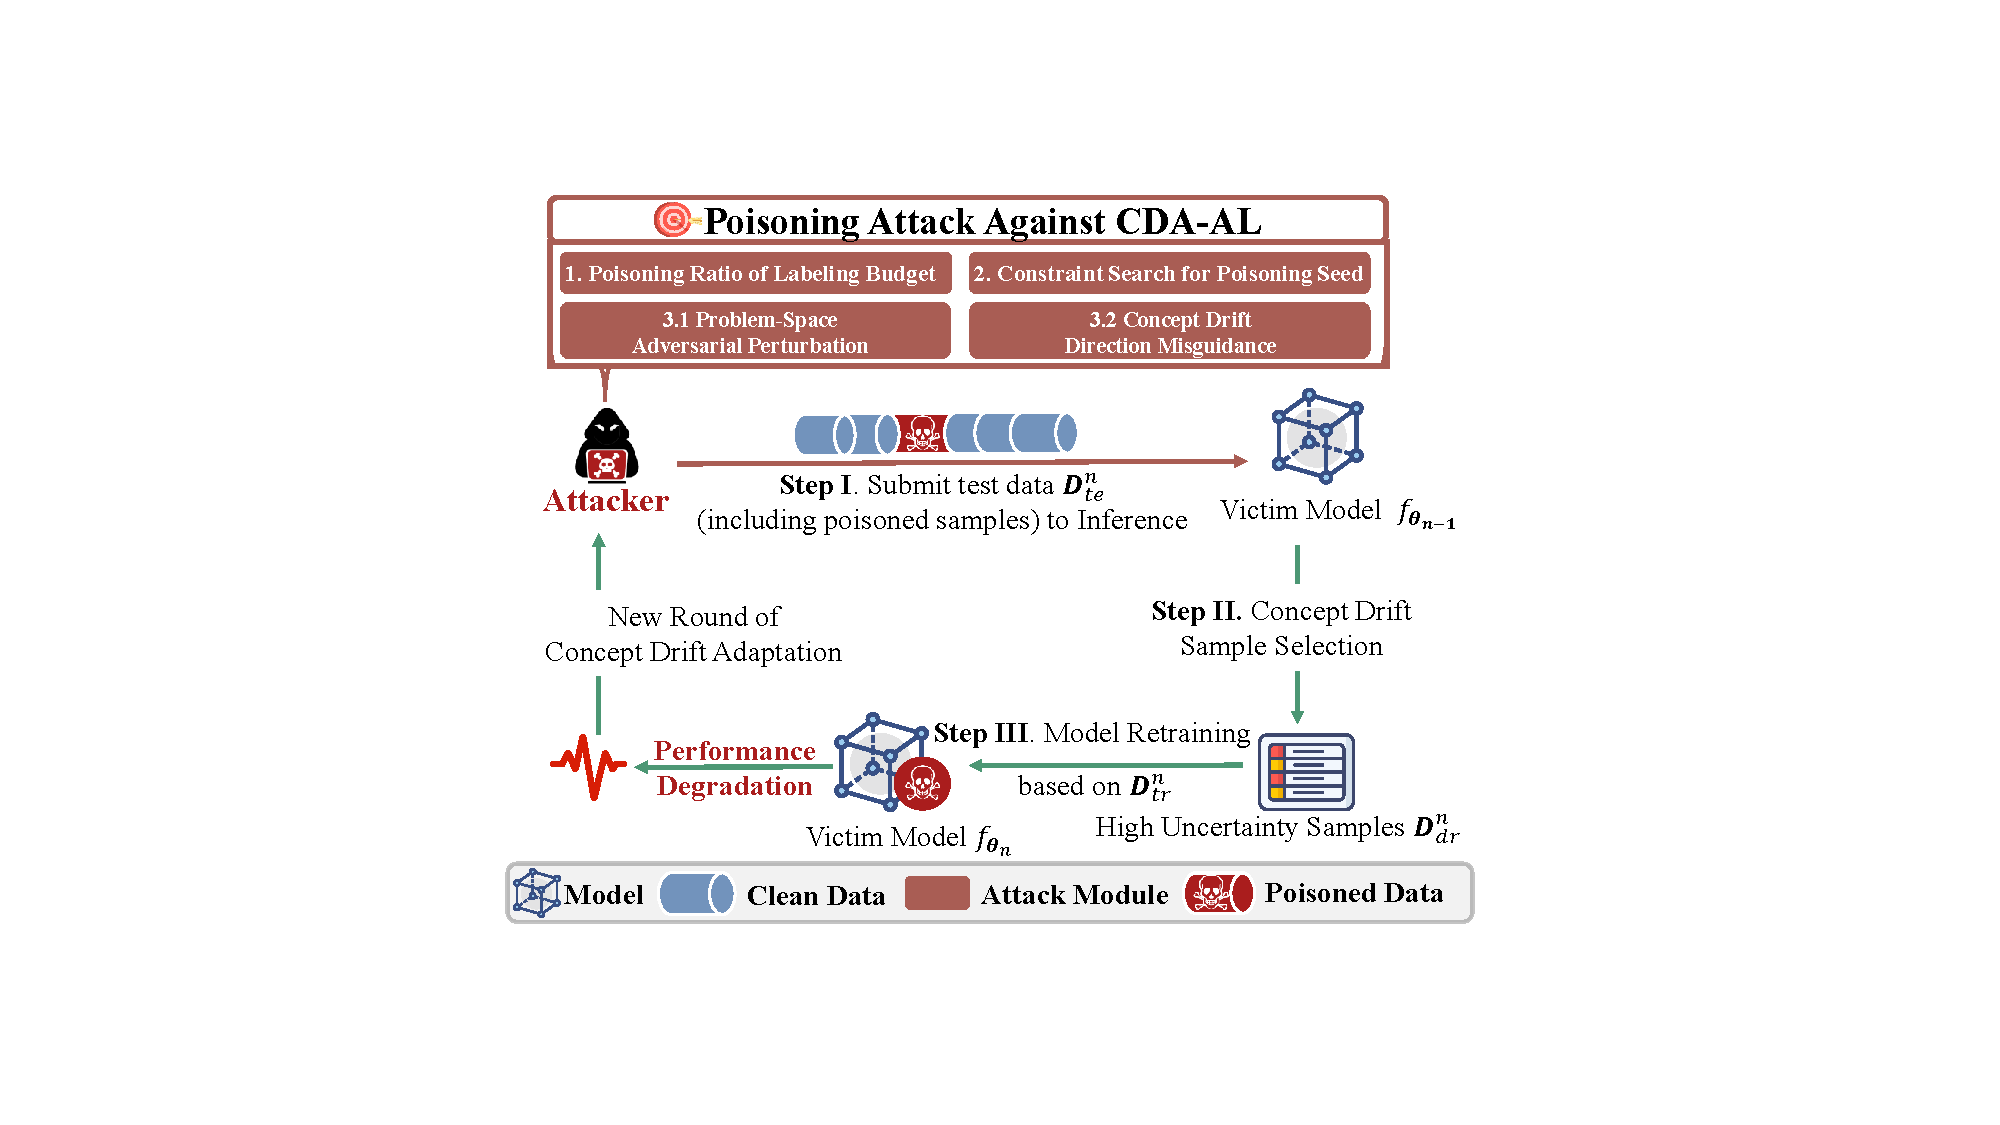
\includegraphics[width=\linewidth,keepaspectratio]{Graph/Attack_Method/PACDA_attack_process_2025_6_6_01_07.pdf}
	\caption{Poisoning Attack against CDA-AL}
	\label{fig:Attack Process}
\end{figure}

\section{\pandora}
\label{Sec: Attack Method}

%\subsection{Overview of \pandora}
We present the \pandora framework, illustrated in Figure~\ref{fig:Attack Process}.
The process begins by estimating the required poisoning ratio of the labeling budget based on the specified attack targets.
By injecting poisoned samples into the testing data stream, the attacker determines which knowledge the victim model can or cannot acquire.
Subsequently, we search the testing data stream to identify potential poisoning seeds.
Based on the identified poisoning seeds, \pandora generates poisoned samples through adversarial perturbations in the problem space, further enhancing the attack effectiveness by misleading the direction of concept drift.
Ultimately, \pandora exhausts the victim model’s labeling budget, preventing effective learning of the attack target.

%\subsection{Detailed Design of \pandora}
%\label{Sec: Detailed Design of PACDA}

We demonstrate the design of the \pandora method by using a specific concept drift cycle $n$ as an example, executing the same attack procedure in every concept drift cycle.
In concept drift cycle $n$, the complete testing dataset collected by the victim model is denoted as $\bm{D}_{te}^{n} \in \mathbb{R}^{N \times d}$ (with N samples in d dimensions).
The attack target sample $\bm{\mathrm{x}}_{tar}$ is a concept drift sample of the testing data $\bm{D}_{te}^{n}$. 
The victim model is denoted as $f_{\bm{\theta}_{n-1}}$, and its labeling budget is represented by $\beta$.
Notably, at the start of concept drift cycle $n$, the victim model is derived from the model updated at the end of concept drift cycle $n-1$. Therefore, the model parameters at this stage are denoted as $\bm{\theta}_{n-1}$.
The victim model performs uncertainty quantification on the collected testing data and ranks the samples accordingly.
The top $\beta$ samples with the highest uncertainty ranking are selected for manual analysis to obtain the concept drift data $\bm{D}_{dr}^{n} \in \mathbb{R}^{\beta \times d}$ (with $\beta$ samples in d dimensions).

%\subsection{Attack Value Assessment}
%\label{Sec: Attack Value Assessment}
%The \pandora is essentially a resource-exhaustion attack that targets the labeling budget of the victim model.
%However, the attacker also faces similar risks of resource exhaustion.
%For example, resources may be wasted if the attacker chooses a attack target already in the training data.
%A failed attack prevents the attacker from obtaining any reward and incurs substantial attack costs.
%Consequently, the attacker must carefully assess whether the attack targets are worth attacking.
%This decision is based on the accuracy of the victim model’s prediction of the attack targets.
%Samples not present in the training data are more likely to be misclassified, making this a strong indicator of attack value.
%The attacker can leverage the victim model to make this determination.
%If the predicted label $\overline{y}_{i}$ of $\bm{\mathrm{x}}_{tar}$ from the victim model $f_{\bm{\theta}_{n-1}}$ differs from the ground-truth label $y_{i}$, the attack target $\bm{\mathrm{x}}_{tar}$ is likely to be of high attack value.

\subsection{Surrogate Model Training}
Since the attacker cannot access the internal information of the victim model to perform uncertainty estimation under the black-box threat model, \pandora trains a surrogate model to provide guidance for the generation of poisoned samples.
First, the attacker cannot query the victim model for sample uncertainty scores. 
In this scenario, the adversary is restricted to accessing only the predicted labels or the output probability distribution generated by the victim model.
Other information, such as sample uncertainty, must be obtained through the surrogate model.
So we propose a surrogate model construction method based on knowledge distillation, where the surrogate model’s parameters $\bm{\theta}_{n-1}^{*}$ approximate those of the victim model $\bm{\theta}_{n-1}$.
%The attacker constructs a surrogate model $f_{\bm{\theta}_{n-1}^{*}}$ using the input-output query function $Q$, where the pseudo label set $\overline{Y}$ by querying the victim model  $f_{\bm{\theta}_{n-1}}$ with input data $\bm{D}_{te}^{n-1}$.
%\begin{equation}
%	\begin{aligned}
%		\overline{Y} = Q(\bm{\theta}_{n-1},\bm{D}_{te}^{n-1}) \\
%	\end{aligned}
%\end{equation}

The purpose of the surrogate model is to identify the optimal parameters $\bm{\theta}_{n-1}^{*}$ such that the prediction error between the surrogate model and the victim model is minimized for all inputs $\bm{\mathrm{x}}_{i} \in \bm{D}_{te}^{n-1}$, as shown in Equation~\ref{Surrogate Model Training}.
\begin{equation}
	\begin{aligned}
		\bm{\theta}_{n-1}^{*} = \arg\min_{\bm{\theta}_{n-2}^{*}} \mathcal{L_{\text{dist}}} \left( \bm{\theta}_{n-2}^{*}, \bm{D}_{te}^{n-1} , \bm{\theta}_{n-1} \right)
	\end{aligned}
	\label{Surrogate Model Training}
\end{equation}
Here, $\mathcal{L_{\text{dist}}}$ denotes the distillation loss function, which employs the symmetric Kullback–Leibler Divergence (KLD) to quantify the similarity between the output distributions of the surrogate model and the victim model, and optimizes the parameters of the surrogate model accordingly.
\begin{equation}
	\small
	\begin{aligned}
		\mathcal{L_{\text{dist}}} 
		&= \frac{1}{|\bm{D}_{te}^{n-1}|} \sum_{x_i \in \bm{D}_{te}^{n-1}} \frac{1}{2} \Big[ 
		\mathrm{KLD}\!\left(h(x_i; \bm{\theta}_{n-1})\,\|\,h(x_i; \bm{\theta}_{n-2}^{*} )\right) \\
		&\quad + \mathrm{KLD}\!\left(h(x_i; \bm{\theta}_{n-2}^{*})\,\|\,h(x_i; \bm{\theta}_{n-1})\right) \Big]
	\end{aligned}
	\label{KL-loss}
\end{equation}
Let $\bm{D}_{te}^{n-1}$ denote the set of samples submitted by the attacker.
For a given input $x_i$, $h(x_i; \bm{\theta}_{n-1})$ represents the predictive distribution of the victim model, while $h(x_i; \bm{\theta}_{n-2}^{*})$ denotes the predictive distribution of the surrogate model.
Note that the loss in Equation~\ref{KL-loss} consists of two KLD terms. 
The first term measures the information loss when the predictive distribution of the victim model is approximated by the surrogate model. 
The second term quantifies the reverse discrepancy, capturing how well the surrogate model’s predictions can be explained by the victim model. 
By combining both directions, the symmetric KL divergence mitigates the asymmetry of the standard KLD and provides a more balanced measure of similarity between the two predictive distributions.
%It is important to emphasize that the attacker uses predictive distribution $\overline{Y}$ generated by the victim model $f_{\bm{\theta}_{n-1}}$ as training labels for the surrogate model rather than relying on ground truth labels.
%There are two main reasons for this approach. 
%First, the methods of concept drift adaptation are primarily applied in sensitive domains such as malware detection and industrial security risk analysis, where acquiring ground truth labels is prohibitively expensive.
%Second, the role of the surrogate model $f_{\bm{\theta}_{n-1}^{*}}$ is to approximate the detection capabilities of the victim model $f_{\bm{\theta}_{n-1}}$, but the victim model does not provide correct labels for the entire testing data $\bm{D}_{te}^{n-1}$. 
%As a result, the surrogate model, trained with pseudo-labels, performs more similarly to the victim model.
In addition, with respect to the selection of training data for the surrogate model $\bm{\theta}_{n-1}^{*}$, it is crucial to properly define the query range of the testing data.
In concept drift cycle $n$, the attacker queries the testing data $\bm{D}_{te}^{n-1}$, which is obtained from the previous concept drift cycle.
This is because the victim model has already completed learning from the previous concept drift cycle.
This model is used to quantify the uncertainty of samples in the current concept drift cycle $n$.
Therefore, to ensure that the surrogate model $\bm{\theta}_{n-1}^{*}$ approximates the victim model $\bm{\theta}_{n-1}$, the attacker queries the testing data $\bm{D}_{te}^{n-1}$ and uses the query results to train the surrogate model.


\subsection{Poisoning Ratio of Labeling Budget}
\label{Sec: Surrogate Model Training}
Once the attack target $\bm{\mathrm{x}}_{tar}$ is determined, the \pandora begins by estimating the poisoning ratio of the labeling budget that needs to be exhausted from the victim model.
The attacker makes decisions based on the uncertainty ranking of the attack target $\bm{\mathrm{x}}_{tar}$.
If the uncertainty ranking $r_{tar}$ of the attack target $\bm{\mathrm{x}}_{tar}$ is higher than the labeling budget boundary $(r_{tar} < r_{\beta})$, the attack target $\bm{\mathrm{x}}_{tar}$ will be selected as a concept drift sample.
It is important to note that a higher uncertainty ranking corresponds to a smaller value of $r_{tar}$.
Then, the attack target $\bm{\mathrm{x}}_{tar}$ will be learned during the retraining process of the victim model.
The gap between the uncertainty ranking of the attack target $\bm{\mathrm{x}}_{tar}$ and the labeling budget boundary represents the primary objective of the attacker’s labeling budget consumption, denoted as $C_{n}$.
It also reflects the minimum requirement for the number of poisoned samples.
When $r_{tar} > r_{\beta}$, it indicates that the attack target $\bm{\mathrm{x}}_{tar}$ will not be selected by the victim model $f_{\bm{\theta}_{n-1}}$.
Nonetheless, the attacker will still generate some poisoned samples, even if the attack target $\bm{\mathrm{x}}_{tar}$ is not selected.
This mitigates potential mismatches between the attacker’s and the victim’s testing data, which could otherwise cause the attacker to overestimate the target’s uncertainty ranking.
Therefore, to ensure reliability, the consumption of the labeling budget is set to a fixed value $\lambda \, (\lambda \ll \bm{D}_{te}^{n})$, determined by the attacker’s computational resources.
Specifically, the amount of budget consumption $C_{n}$ for labeling is as follows:
\begin{align}
	C_{n} =
	\begin{cases} 
		(r_{\beta}-r_{tar}) + 1, \; r_{tar} < r_{\beta} \\
		\lambda , \; r_{tar} > r_{\beta}
	\end{cases}
\end{align}
Furthermore, considering the inherent randomness in sample selection and model training, we introduce an amplification factor to the originally computed label budget consumption $C_{n}$ to mitigate the effects of randomness.
The specific value of this factor is determined by the attacker's computational capabilities.

\subsection{Constraint Search for Poisoning Seed}
The attacker then searches for samples that can be used to exhaust the victim model’s labeling budget $C_{n}$.
These selected samples are referred to as poisoning seed samples.
The poisoning seed data, denoted as $\bm{D}_{seed}^{n} \in \mathbb{R}^{K \times d}$ (with $K$ samples in d dimensions), consists of samples that satisfy the uncertainty criterion defined in Equation~\ref{equncer}.
We denote each row of the testing data as a sample vector $\bm{\mathrm{x}}_{i}$, where $\bm{\mathrm{x}}_{i} = \bm{D}_{te,\,i*}^{n}$,$\forall i \in \{0, \dots, N-1\}$.
The key issue is ensuring that the poisoned samples have high uncertainty, thereby increasing the likelihood that they consume the victim model's labeling budget.
So the uncertainty of these poisoned seed samples must exceed the attack target’s uncertainty, as shown in Equation~\ref{equncer}.
\begin{equation}
	\begin{aligned}
		uncer(f_{\bm{\theta}_{n-1}} \left( \bm{\mathrm{x}}_{i} \right)) > uncer(f_{\bm{\theta}_{n-1}} \left( \bm{\mathrm{x}}_{tar} \right))
	\end{aligned}
	\label{equncer}
\end{equation}
%Inspired by Yang et al. and Chen et al., who represent sample uncertainty by measuring the similarity between testing and training data~\cite{2021-Usenix-CDAE,2023-Usenix-chenyizhen}, we find that newly appearing concept drift samples always inherently exhibit high uncertainty.
%This is primarily because of their low similarity to the existing training data.
%Therefore, \pandora exploits the inherent high uncertainty of concept drift samples to get poisoned seed data.
Furthermore, it is crucial to ensure that the poisoned samples exhaust the victim model’s labeling budget without enhancing its concept drift adaptation capability.
For instance, incorporating novel malware samples into the poisoning seed data may improve the victim model’s ability to detect malicious behavior, thereby undermining the attacker’s objective of causing misclassification of the attack target $\bm{\mathrm{x}}_{tar}$.
Therefore, the attacker must exclude malware samples from the poisoning seed data to avoid reducing the attack effectiveness on the target $\bm{\mathrm{x}}_{tar}$.
In addition, similarity-based filtering can be employed to prevent the inclusion of samples similar to the attack target $\bm{\mathrm{x}}_{tar}$ in the poisoned samples.
\begin{equation}
	\begin{aligned}
		(y_{j} \neq y_{tar}) \land [sim(\bm{\mathrm{x}}_{j},\bm{\mathrm{x}}_{tar})< \tau]
	\end{aligned}
	\label{E6}
\end{equation}
Each row of the poisoning seed data $\bm{D}_{seed}^{n}$ is denoted as a sample vector $\bm{\mathrm{x}}_{j}$, where $\bm{\mathrm{x}}_{j} = \bm{D}_{\text{seed}}^{n}[j,:]$,$\forall j \in \{0, \dots, K-1\}$.
The constraint condition applied to each sample vector $\bm{\mathrm{x}}_{j}$ is defined in Equation~\ref{E6}.
Samples that do not satisfy this condition are removed from the poisoning seed data $\bm{D}_{seed}^{n}$.
Finally, the refined poisoning seed data is sorted in descending order of uncertainty, with the sample at index 0 having the highest uncertainty.

%\subsection{Poisoning Seed Uncertainty Attribution}
%After obtaining the poisoned seed samples $\bm{D}_{seed}^{n}$, we aim to interpret their uncertainty to facilitate the subsequent poisoned sample generation by expanding the space of manipulable uncertainty rankings.
%Given the need to accommodate various models for CDA-AL, our uncertainty attribution method should be model-agnostic.
%Moreover, to effectively construct poisoned samples with high uncertainty, the explanation should operate at the feature level.
%Although standard conformal prediction methods can provide interpretable uncertainty estimates through credibility scores, they are unable to offer feature-level explanations of uncertainty.
%Therefore, we adopt a shapley additive explanations (SHAP) based approach for feature level attribution of sample uncertainty.
%The fundamental concepts of SHAP are provided in Appendix~\ref{Sec: Shapley Additive Explanations}.
%We employ a standardized permutation-based SHAP method to interpret sample uncertainty, ultimately getting an uncertainty attribution matrix for the samples.
%%We utilize a standardized permutation-based SHAP method to interpret sample uncertainty, approximating shapley values by iterating through permutations of input features.
%%This model-agnostic explainer ensures local accuracy (additivity) by iterating completely through an entire permutation of the features in both forward and reverse directions (antithetic sampling).
%Since the objective of \pandora is to prevent the victim model from learning the attack target $\bm{\mathrm{x}}_{tar}$, the generated poisoned samples must suppress the model’s ability to adapt to concept drift.
%To achieve this, samples outside the labeling budget are selected as targets for uncertainty attribution.
%Their lower importance relative to in-budget samples helps avoid inadvertently strengthening the model’s adaptation capabilities.
%The attacker applies uncertainty feature attribution on the testing data outside the labeling budget, denoted as $\bm{D}_{shap}^{n}$ ($\bm{D}_{shap}^{n} = \bm{D}_{te}^{n} \setminus \bm{D}_{dr}^{n}$).
%These samples are then sorted in descending order based on their uncertainty scores.
%\begin{equation}
%	\begin{aligned}
%		 \bm{V}_{shap} = SHAP (\bm{D}_{tr}^{n-1},UncerSort(\bm{D}_{shap}^{n})) \\
%	\end{aligned}
%\end{equation}
%$\bm{V}_{shap}$ represents the matrix of uncertainty feature attributions for data $\bm{D}_{shap}^{n}$.
%$\bm{\mathrm{v}}_{i}$ denotes the feature attribution vector of a specific sample, while $v_{i,j}$ indicates the impact of a particular feature on the uncertainty of the given sample.

\subsection{Poisoned Sample Generation}
\label{Sec: Poisoned Sample Generation}
The poisoned seed samples $\bm{D}_{seed}^{n}$ is incorporated into the victim model’s training dataset due to its high uncertainty.
However, the seed samples obtained via the constrained search strategy may not fully satisfy the required labeling budget consumption $C_{n}$.
Consequently, attack targets will still be selected and labeled manually, leading to a failure of \pandora.
To ensure the attack effectiveness, the attacker must generate an additional batch of poisoned samples such that the total number of poisoned samples is greater than or equal to the labeling budget consumption $C_{n}$.
The poisoned sample generation process consists of two parts.
The first part generates poisoned samples based on high-uncertainty poisoning seeds to exhaust the labeling budget, thereby preventing the victim model from learning samples directly related to the attack targets.
The second part constructs poisoned samples using shapley additive explanations to misguide the direction of concept drift, with the aim of eliminating samples that are implicitly related to the attack targets within the labeling budget.
The combination of the two parts prevents the victim model from effectively learning the attack targets while also hindering its understanding of the correct direction of concept drift.

%\subsubsection{Selection of Poisoned Sample Generation Strategy}
%\label{Sec: Selection of Poisoned Sample Generation Strategy}
%We propose two poisoned sample generation strategies: Strategy I, which is based on problem-space perturbation, and Strategy II, which leverages Shapley additive explanations.
%Both strategies aim to generate poisoned samples, thereby leading to misclassification of the attack target $\bm{\mathrm{x}}_{tar}$.
%However, the two strategies are suitable for different attack scenarios.
%
%However, the two strategies are suitable for different types of attack targets.
%Strategy I prevents the victim model from learning specific knowledge about the attack target $\bm{\mathrm{x}}_{tar}$ by constructing poisoned samples without introducing incorrect concept drift information.
%It focuses solely on preventing the victim model from learning the attack target $\bm{\mathrm{x}}_{tar}$ while minimizing its impact on the model’s ability to adapt to concept drift.
%In contrast, Strategy II prevents the victim model from acquiring knowledge about the attack target $\bm{\mathrm{x}}_{tar}$ and introduces misleading information about concept drift into the training process.
%Although this reduces the model’s ability to adapt to true concept drift in the testing data, it does not cause a significant drop in overall performance, as indicated by the F1 score in Table~\ref{tab:Attack Effectiveness}.
%
%In terms of strategy selection, Strategy I is better suited for attack targets that are inherently challenging to learn, typically those exhibiting a high degree of concept drift.
%Conversely, when the attack targets is relatively easy to learn due to weak concept drift, strategy II is employed to enhance the effectiveness of the attack.
%Finally, we ensure that, regardless of the degree of concept drift exhibited by the attack targets, the victim model fails to learn the attack target due to its inability to efficiently allocate the limited labeling budget, ultimately leading to the misclassification of the attack targets.

\subsubsection{Problem-Space Adversarial Perturbation}
\label{Sec: Strategy I-Problem-Space Perturbation}
Adversarial perturbation is particularly effective for rapidly and cost-efficiently adjusting the uncertainty rankings of the testing data.
%For instance, consider a sample $\bm{\mathrm{x}}_{A}$ from the poisoning seed data $\bm{D}_{seed}^{t+1}$.
%Let the attack target be denoted by $\bm{\mathrm{x}}_{tar}$.
%Their respective uncertainty rankings are $r_{A}$ and $r_{tar}$, respectively, and their uncertainty scores are $u_{A}$ and $u_{tar}$ ,with $u_{A} > u_{tar}$.
%By applying problem space perturbation to sample $\bm{\mathrm{x}}_{A}$, we can generate a poisoned sample that maintains a similar uncertainty level $u_{A}$.
The problem space perturbation strategy refers to modifying the samples in the poisoning attack seed data $\bm{D}_{seed}^{n}$ to generate new poisoned samples without altering the features of these samples.
We denote each row of the attack seed data $\bm{D}_{seed}^{n}$ as a sample vector $\bm{\mathrm{x}}_{k}$, where $\bm{\mathrm{x}}_{k} = \bm{D}_{\text{seed}}^{n}[k,:]$,$\forall k \in \{0, \dots, M-1 \}$.
Due to the need for attack stealth, the samples generated by problem space perturbation must minimize the impact on other concept drift samples. 
Therefore, we select the $\epsilon$ least uncertain samples from the poisoned seed sample set for problem space perturbation. 
The smaller $\epsilon$ is, the lesser the impact on existing concept drift samples.
In this paper's subsequent attack effectiveness evaluation, we set $\epsilon$ to 5, which accounts for 0.025 of the labeling budget.
A perturbation in the problem space is applied to these samples $\bm{\mathrm{x}}_{k}$, $k \in \{0, \dots,  \epsilon-1 \}$ , resulting in a new dataset denoted as $\bm{D}_{\alpha}^{n}$.
$\alpha$ denotes the problem-space perturbation operations.
This strategy ensures that the newly generated poisoned samples exhibit high uncertainty, thereby maintaining their potential to exhaust the victim model’s labeling budget and increase the uncertainty ranking of the attack target $r_{tar}$ beyond the labeling budget boundary (i.e., $r_{tar} > r_{\beta}$).
\begin{table}[h!]
	\caption{Problem-Space Perturbation Operations}
	\label{tab: List of Problem Space Perturbation Operations}
	\setlength{\tabcolsep}{5.8pt}
	\begin{center}
		\scalebox{1.0}{
			\begin{tabular}{cc}
				\toprule
				\textbf{Dataset} & \textbf{Perturbation Operations ($\alpha$)}\\
				\midrule
				APIGraph & Rename method names to meaningless identifiers  \\ 
				\specialrule{0.05em}{1pt}{1pt}
%				APIGraph & Modify image and other resource files     \\ 
%				\specialrule{0.05em}{1pt}{1pt}
%				BODMAS & Modify the system API function names   \\
%				\specialrule{0.05em}{1pt}{1pt}
				BODMAS & Dynamically adjust the size of the DOS STUB space  \\
				\specialrule{0.05em}{1pt}{1pt}
%				MNIST & Add Gaussian noise to the image pixels  \\
%				\specialrule{0.05em}{1pt}{1pt}
				MNIST & Apply sharpening to enhance the edges of the image  \\
				\specialrule{0.05em}{1pt}{1pt}
%				SPAM & Remove non-essential words \\
%				\specialrule{0.05em}{1pt}{1pt}
				SPAM & Insert random symbols or additional spaces  \\
				\bottomrule
		\end{tabular}}
	\end{center}
\end{table}

The reason is that machine learning models, during the feature extraction process, often ensure that non-critical perturbations $\alpha$ in the data do not affect the features in order to construct robust representations.
Therefore, when the attacker adjusts the non-essential information of a sample, the sample is altered, but its features remain unchanged.
Since existing uncertainty quantification methods are based on sample features, altering the problem space does not reduce the sample's uncertainty, ensuring that the labeling budget can be exhausted.
For example, in software applications, when key information such as permissions and API calls is extracted as features, elements like coding style and redundant code have no direct relationship with these critical features.
Examples of problem space perturbations in different domains can be found in Table~\ref{tab: List of Problem Space Perturbation Operations}.
All perturbation operations preserve the original labels of the poisoned seed samples.
The perturbation operation in the problem space is infinite, allowing for generating a sufficient number of poisoned samples.
Thus, by leveraging high-uncertainty seed samples $\bm{D}_{seed}^{n}$ and the problem space perturbation strategy, the attacker can generate poisoned samples $\bm{D}_{\alpha}^{n}$ to meet the victim model's labeling budget consumption $C_{n}$.

\subsubsection{Concept Drift Direction Misguidance}
\label{Sec: Strategy II: Feature-Space Perturbation}
The uncertainty of poisoned samples generated through problem-space adversarial perturbation is limited by the uncertainty of the seed samples from $\bm{D}_{seed}^{n}$.
Thus, it is difficult to affect samples with higher uncertainty than the poisoned seed samples.
If the portion of the labeling budget with higher uncertainty than the poisoning seed samples includes samples that affect the misclassification of the attack targets (e.g., malware sharing similar vulnerabilities with the target), the attack effectiveness may be reduced.
Since these high-uncertainty concept drift samples are beyond the control of the attacker, we need to construct poisoned samples with higher uncertainty than the poisoned seed samples to mislead the victim model in its learning of the direction of concept drift.
Building on the insights of Ledda et al., who employed perturbation search techniques to identify minimal perturbations that alter a sample's uncertainty~\cite{Ledda_2023_ICCV}, we aim to manipulate the uncertainty of poisoned samples.
However, while their method aims to reduce uncertainty, CDA-AL instead selects samples with high uncertainty.
Moreover, Ledda et al.’s approach relies on gradient information and is therefore inapplicable to CDA-AL, since our model assumes no access to parameters~\cite{Ledda_2023_ICCV}.
To address this limitation, we propose a shapley additive explanations (SHAP) based uncertainty maximization strategy that relies solely on predicted scores.
We first conduct uncertainty attribution on the samples to identify features that can increase their uncertainty.
Given the need to accommodate various models for CDA-AL, our uncertainty attribution method should be model-agnostic.
Moreover, to effectively construct poisoned samples with high uncertainty, the explanation should operate at the feature level.
Although standard conformal prediction methods can provide interpretable uncertainty estimates through credibility scores, they are unable to offer feature-level explanations of uncertainty.
Therefore, we adopt a SHAP based approach for feature level attribution of sample uncertainty.
The fundamental concepts of SHAP are provided in Appendix~\ref{Sec: Shapley Additive Explanations}.
We employ a standardized permutation-based SHAP method to interpret sample uncertainty, ultimately getting an uncertainty attribution matrix for the samples.

In selecting the analysis targets for uncertainty attribution, it is important to note that since the objective of \pandora is to prevent the victim model from learning the attack target  $\bm{\mathrm{x}}_{tar}$, the generated poisoned samples must hinder the model’s ability to adapt to concept drift.
To achieve this, samples outside the labeling budget are selected as targets for uncertainty attribution.
Their lower importance relative to in-budget samples helps avoid inadvertently strengthening the model’s adaptation capabilities.
the testing data outside the labeling budget, denoted as $\bm{D}_{shap}^{n}$ ($\bm{D}_{shap}^{n} = \bm{D}_{te}^{n} \setminus \bm{D}_{dr}^{n}$).
Then We compute the uncertainty attribution matrix of $\bm{D}_{shap}^{n}$, as shown in Equation~\ref{shap-uncer}.
%We utilize a standardized permutation-based SHAP method to interpret sample uncertainty, approximating shapley values by iterating through permutations of input features.
%This model-agnostic explainer ensures local accuracy (additivity) by iterating completely through an entire permutation of the features in both forward and reverse directions (antithetic sampling).
\begin{equation}
	\begin{aligned}
		\bm{V}_{shap} = SHAP (\bm{D}_{tr}^{n-1},UncerSort(\bm{D}_{shap}^{n})) \\
	\end{aligned}
	\label{shap-uncer}
\end{equation}
$\bm{V}_{shap}$ represents the matrix of uncertainty feature attributions for data $\bm{D}_{shap}^{n}$.
%$\bm{\mathrm{v}}_{i}$ denotes the feature attribution vector of a specific sample, while $v_{i,j}$ indicates the impact of a particular feature on the uncertainty of the given sample.
%It is worth noting that the uncertainty attribution matrix $\bm{V}_{shap}$ allows samples originally outside the labeling budget to be shifted into the budget through feature-space perturbation.
%Consequently, we eliminate the dependence on high-uncertainty seed samples $\bm{D}_{seed}^{n}$.
%It enhances \pandora’s robustness by preventing the victim model from acquiring accurate knowledge of actual concept drift samples, instead introducing misleading concept drift information into the victim model.
%So, the attacker can operate in two different attack modes based on the cost the attack service purchaser is willing to pay.
%The attacker can choose to use the problem space perturbation strategy alone. 
%This approach is low-cost, but the attack success rate on some attack targets cannot be guaranteed.
%If the attacker has sufficient computational resources and aims for a higher attack success rate, they can generate poisoned samples by applying feature space perturbations.
We denote each row of the uncertainty attribution matrix as a vector $\bm{\mathrm{v}}_{i}$, where $\bm{\mathrm{v}}_{i} =\bm{V}_{\text{shap}}[i,:]$,$\forall i \in \{0, \dots, N-1 \}$.
Based on the uncertainty feature attribution vector $\bm{\mathrm{v}}_{i}$ for each sample, the attacker identifies the set of feature indices $\bm{I}_{shap}$ that have the greatest impact on increasing uncertainty.
The computation of the feature index vector $\bm{I}_{shap}$ is shown in Equation~\ref{mask}.
\begin{equation}
	\begin{aligned}
		\bm{I}_{shap} = \{ argsort(\bm{\mathrm{v}_{i}})[0:d-1]  \} \\
		\end{aligned}
	\label{mask}
\end{equation}
$d$ denotes the dimension of the feature vector for each sample.
The sorting function ranks feature indices based on their influence on sample uncertainty, such that features contributing more to increased uncertainty are assigned smaller index values.  
Therefore, the attacker can focus on modifying features with lower index values to effectively amplify uncertainty.
%As shown in Figure 4, the Force plot of the uncertainty feature attribution vector $\bm{\mathrm{v}}_{i}$ is ordered by the $\bm{I}_{shap}$ index.
%Red indicates features that increase the sample's uncertainty, while blue represents features that decrease it.
%The features closer to the center significantly impact uncertainty, corresponding to the lower-indexed parts of $\bm{I}_{shap}$.
%Modifying the features corresponding to the indices of the blue region will increase the sample uncertainty, as shown in Figure~\ref{fig:SHAP}.
We selected the top 2\% of features based on their indices for modification.
Since the uncertainty-based SHAP attribution provides a linear approximation of the model's predictive uncertainty, modifying the key features with the highest attribution values increases the sample's overall uncertainty.
%\begin{figure}[h!]
%	\centering
%	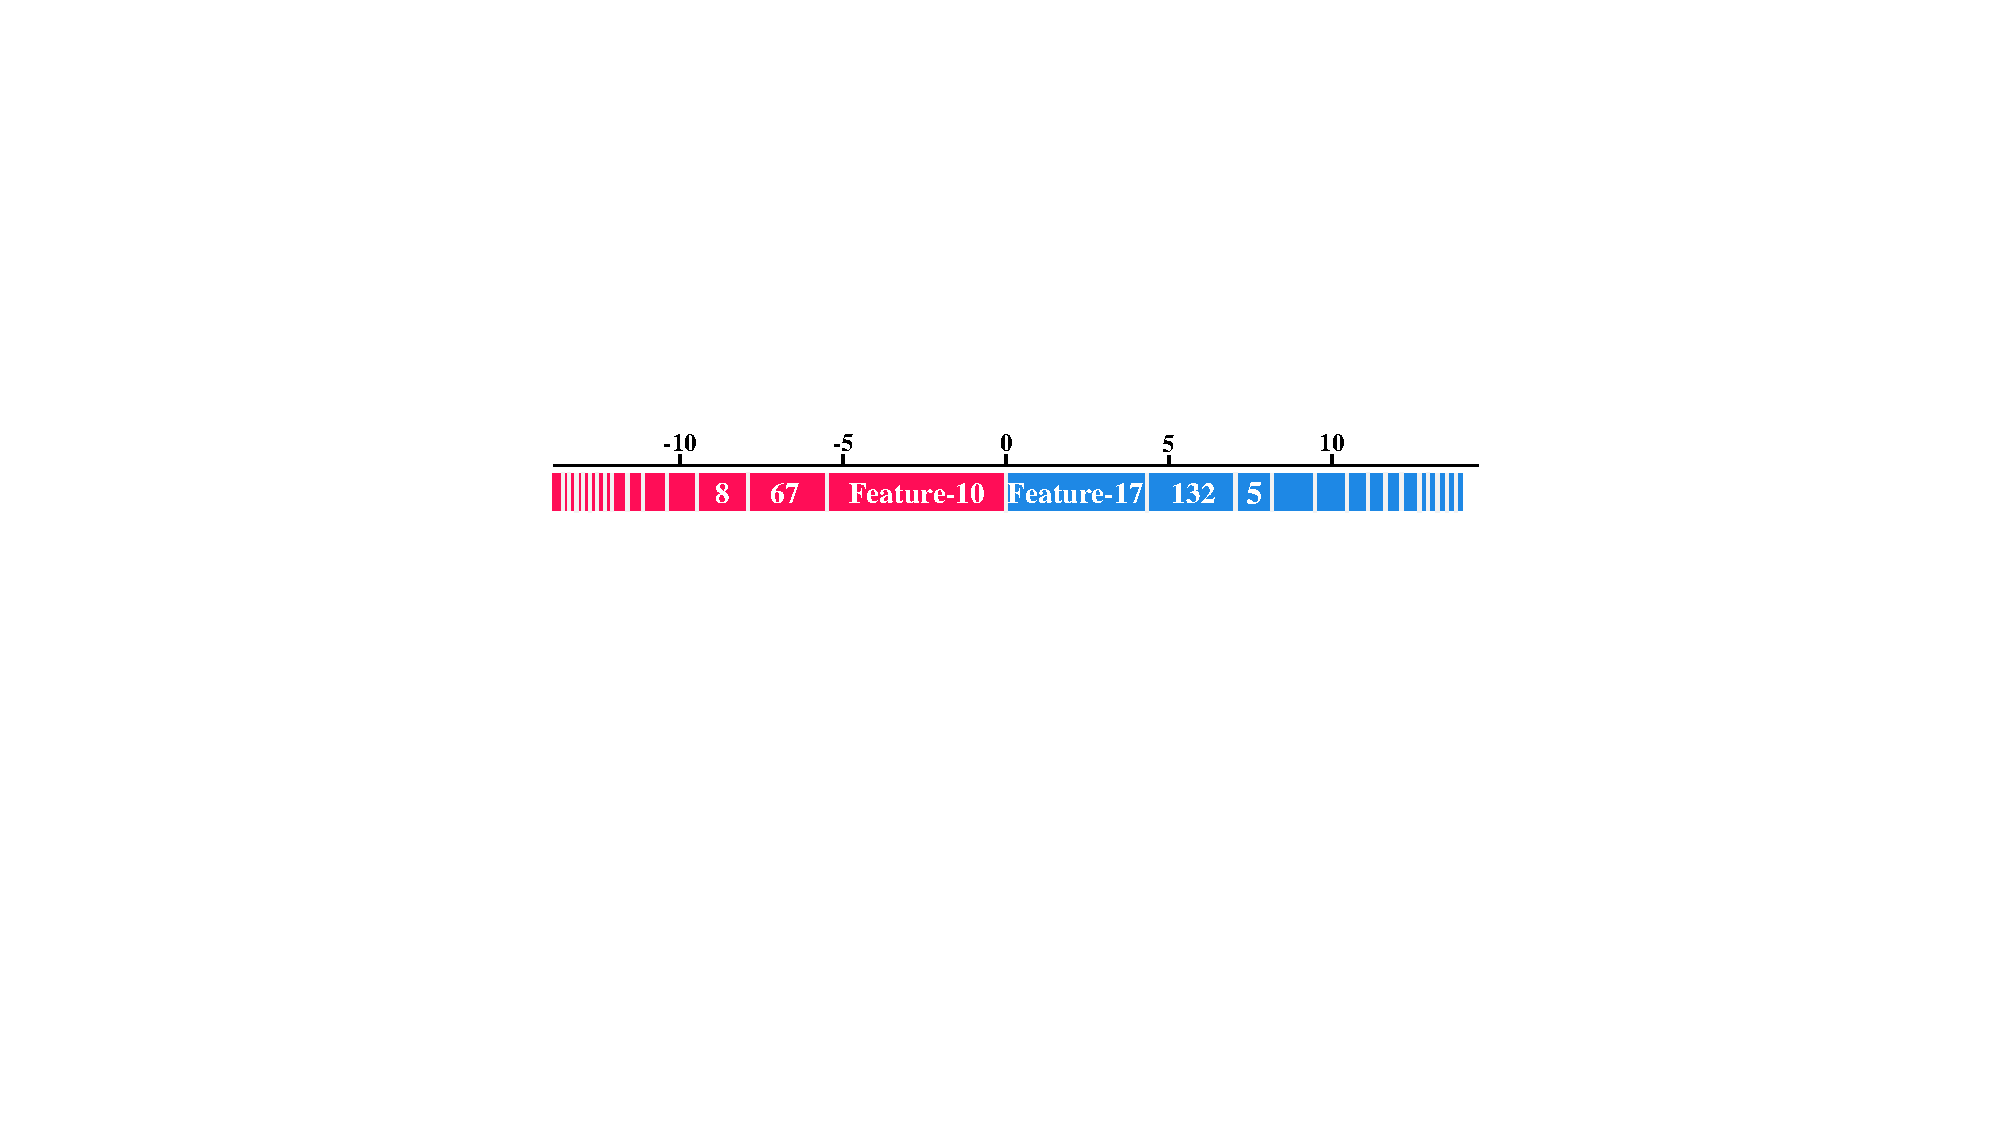
\includegraphics[width=\linewidth,keepaspectratio]{Graph/Evaluation/shap.pdf}
%	\caption{SHAP-based Sample Uncertainty Attribution}
%	\label{fig:SHAP}
%\end{figure}

A sample from the APIGraph dataset is taken as an example, and its features are represented as 0-1 vectors.
This feature modification corresponds to adjusting the API call patterns in the actual application.
Since the poisoned samples are intended to consume the labeling budget, the impact of the API calls on the program's functionality does not need to be considered.
Moreover, the modifications only reduce software API calls without introducing additional sensitive behaviors, thereby preserving the original label of the sample.
For data in other domains, we replace the values of the important features with the corresponding values from samples with high uncertainty.
The perturbed samples generated in this manner are considered as a new set of poisoned attack samples $\bm{D}_{shap}^{n}$.
The attacker can further amplify the set by applying problem space perturbation to the poisoned samples $\bm{D}_{shap}^{n}$ to enhance their impact on the victim model.

%Moreover, the number of poisoned samples only needs to be sufficient to consume the victim model's labeling budget. 
%Consequently, they constitute only a small fraction of the training data.
%For example, in the real-world APIGraph~\cite{2020-CCS-APIGraph} data, poisoned samples generated in a single attack account for only 1\% of the training data.
%In addition to the stealth provided by the low poisoning ratio, all poisoned samples retain correct labels without any label flipping.